% =========================================================
% CHAPTER 3 — PROBLEM FORMULATION AND OBJECTIVES
% =========================================================

\chapter{Problem Formulation and Objectives}

\section{Problem Statement}

The contemporary digital landscape is heavily characterized by an increasing asymmetry in information and control between service providers and end-users. While web technologies have advanced to offer dynamic, highly personalized user experiences, they have simultaneously enabled sophisticated mechanisms for user manipulation and exploitation. This manipulation predominantly manifests in two distinct but related forms: dark patterns and phishing attacks. 

Dark patterns represent a deliberate subversion of human-computer interaction (HCI) principles. Rather than optimizing for usability and transparency, these user interfaces are meticulously engineered to exploit human cognitive biases, thereby nudging or coercing users into actions that are disproportionately beneficial to the service provider. Examples include forced continuity in subscription models, hidden costs that only appear at the final stage of a checkout process, and confirmshaming that guilt-trips users into opting into data collection. The fundamental problem is that conventional security mechanisms—such as web firewalls and antivirus software—treat dark patterns as benign content because they are structurally identical to legitimate UI components and are hosted on legitimate domains.

Conversely, phishing attacks represent a more overt security threat wherein malicious entities masquerade as trustworthy entities to extract sensitive credentials, such as banking passwords and personal identification information. Traditional anti-phishing mechanisms rely heavily on static blacklists, URL reputation scoring, and domain age analysis. However, modern phishing campaigns utilize zero-day domains, perfectly cloned user interfaces, and contextually persuasive language, rendering static heuristics ineffective.

A critical vulnerability in modern AI-based threat detection systems is the high incidence of false positives on legitimate authentication forms. Legitimate sign-in and credential verification interfaces (such as GitHub, Google, LinkedIn, and PayPal) heavily feature critical security keywords like "login", "password", "verify", "secure", and "account". In standard sequence classification models, the presence of these keywords triggers high-confidence phishing classifications (>0.95), even when the domain is fully trusted and legitimate. This lack of domain-aware context leads to alert fatigue, prompting users to disable security controls and exposing them to real attacks.

The core problem addressed by this project is the lack of a unified, real-time, context-aware detection system capable of identifying both manipulative interface designs (dark patterns) and fraudulent semantic intents (phishing) directly within the user's browsing environment without falsely flagging trusted resources. Existing solutions are either heavily siloed—focusing solely on phishing while ignoring dark patterns—or rely on post-hoc analysis rather than real-time intervention. There is a critical need for an intelligent client-side agent that can continuously parse the Document Object Model (DOM), verify domain reputations, analyze text heuristics, and run transformer-based inference asynchronously to highlight malicious elements while keeping legitimate sites clean.

\section{Objectives of the Project}

The primary objective of this project is to conceptualize, design, and implement an AI-powered browser extension, named ``DESIGN TO DECEIVE'', capable of detecting and mitigating dark patterns and phishing attempts in real-time. To achieve this overarching goal, the project is divided into the following specific objectives:

\begin{enumerate}
    \item \textbf{To develop a dynamic DOM scanning architecture:} Design a lightweight content script capable of traversing the web page's Document Object Model in real-time, utilizing \texttt{MutationObserver} APIs to handle dynamically loaded content in Single Page Applications (SPAs) without causing significant main-thread blocking or rendering latency.
    \item \textbf{To implement a robust NLP-based classification backend:} Engineer a high-performance RESTful API using FastAPI to serve fine-tuned RoBERTa (Robustly Optimized BERT Pretraining Approach) transformer models. This backend must be capable of receiving batched text payloads from the extension and performing binary or multi-class semantic classification with minimal inference delay.
    \item \textbf{To construct distinct detection pipelines for multifaceted threats:} Train and deploy specialized NLP models for different threat vectors: one optimized for identifying coercive and manipulative language indicative of dark patterns, and another fine-tuned on phishing corpora to detect deceptive social engineering tactics.
    \item \textbf{To engineer an intuitive, non-disruptive user interface for threat visualization:} Develop a visual highlighting mechanism and a contextual tooltip system that overlays onto the web page, alerting users to specific deceptive elements. Additionally, create a centralized cybersecurity dashboard within the extension popup to display aggregated risk scores, confidence metrics, and historical detection data.
    \item \textbf{To implement a hybrid, context-aware decision engine:} Design a decision pipeline that integrates URL reputation checks, domain whitelisting, urgency keyword matching, and transformer inference to differentiate between trusted authentication pages and malicious credential harvesting attempts.
    \item \textbf{To ensure real-time performance and privacy preservation:} Optimize the communication overhead between the browser extension and the backend inference server using asynchronous message passing and payload batching, ensuring that the detection pipeline operates within acceptable latency thresholds suitable for active browsing.
\end{enumerate}

% =========================================================
% CHAPTER 4 — SYSTEM ARCHITECTURE AND METHODOLOGY
% =========================================================

\chapter{System Architecture and Methodology}

\section{Proposed Methodology}

The proposed methodology for the ``DESIGN TO DECEIVE'' framework relies on a hybrid architecture combining client-side DOM extraction with server-side heavy-duty NLP inference. The methodology is structured around a continuous, real-time processing loop that executes asynchronously alongside the user's browsing activities.

Unlike traditional static analysis tools that evaluate an entire webpage's source code at load time, our approach adopts a dynamic, element-wise analysis strategy. As the user navigates a website, the extension selectively targets specific HTML elements that are historically prone to containing manipulative text—such as buttons, hyperlinks, form labels, and modal dialogs. The text content and the current page URL are extracted, cleaned of HTML markup, and transmitted to the centralized machine learning backend.

At the backend, the system implements a hybrid decision logic. First, the page domain is extracted and verified against a trusted whitelist. If the domain is trusted, the classification thresholds are tightened and standard input fields are bypassed to prevent false alerts. Second, the domain is checked against URL reputation rules (such as suspicious TLDs, excessive hyphens, and token-based brand spoofing). Third, the text is scanned for contextual triggers like urgency language. Finally, the text is processed by fine-tuned RoBERTa sequence classification models to establish a contextual threat signature.

The classification result, along with its confidence score, risk tier (None, Low Risk, Medium Risk, High Risk), and a generated explanation, is returned to the extension. The extension then modifies the local DOM to inject visual indicators—specifically, CSS-based highlights and interactive tooltips—exclusively for High Risk detections, preventing interface clutter on benign pages.

\section{System Architecture}

The system architecture follows a decoupled, client-server paradigm, specifically chosen to offload the computationally expensive transformer inference from the resource-constrained browser environment to a dedicated backend server.

The architecture comprises three primary tiers:

\begin{enumerate}
    \item \textbf{The Client Tier (Chrome Extension):} Operating directly within the user's browser, this tier consists of Content Scripts (for DOM manipulation and extraction), a Background Service Worker (acting as the central event router and state manager), and the User Interface components (Popup Dashboard and injected Tooltips).
    \item \textbf{The Middleware Tier (FastAPI Engine):} A high-throughput Python-based web server responsible for handling incoming HTTP requests, managing asynchronous batching, and routing payloads to the appropriate NLP models and heuristic modules.
    \item \textbf{The Inference Tier (Hybrid Engine and RoBERTa Models):} The core intelligence of the system, combining pre-trained language models loaded into memory via PyTorch, a domain reputation evaluator, and a heuristic rule compiler to calculate contextual threat bands.
\end{enumerate}

\section{Working Principle}

The working principle of the system can be delineated into five sequential phases:

\textbf{Phase 1: Initialization and Injection.} Upon navigating to a new URL, the browser executes the extension's content script. The script registers event listeners and initializes a \texttt{MutationObserver} to monitor the DOM for structural changes.

\textbf{Phase 2: Extraction and Filtering.} The content script scans the DOM for targeted tags (e.g., \texttt{<a>}, \texttt{<button>}, \texttt{<span>}). It extracts the text, the tag name, and the page URL, generating a local batch of elements with unique identifiers.

\textbf{Phase 3: Payload Transmission.} The content script utilizes the Chrome Messaging API to pass the batched elements to the background service worker, which forwards an asynchronous HTTP \texttt{POST} request to the FastAPI backend.

\textbf{Phase 4: Hybrid Inference and Logging.} The backend receives the payload and processes each element. The domain is parsed and reputation heuristics are run. The backend checks if the domain is whitelisted. If the domain is trusted and the text contains no urgency indicators, the backend skips the ML model pass, logging the bypass. Otherwise, the text is tokenized and evaluated by the RoBERTa model. The final threat level is computed by integrating the ML logits with domain and urgency heuristics. Detections are assigned to risk bands (None, Low, Medium, High). High-confidence alerts are logged as security warnings.

\textbf{Phase 5: Visualization and Alerting.} The service worker receives the response. The content script processes each item: elements categorized as High Risk phishing are visually outlined with a pulsating red CSS border, and mouse hover listeners are registered to render dynamic tooltips. Medium and Low risk classifications are cached for reporting but do not visually alter the webpage layout.

\section{Data Flow Diagram}

To illustrate the flow of data through the system, Data Flow Diagrams (DFDs) have been designed at various abstraction levels.

The Level 0 DFD provides a macroscopic view, showing the user initiating web requests, the browser fetching HTML content, the extension intercepting the DOM along with page URLs, and the interaction with the external NLP API.

The Level 1 DFD breaks down the system into detailed processes: DOM Extraction, Message Routing, HTTP Request Handling, Domain Whitelist Check, URL Reputation Scoring, RoBERTa Tokenization and Inference, Risk Score Normalization, and DOM Modification.

% =========================================================
% CHAPTER 5 — TECHNOLOGY STACK
% =========================================================

\chapter{Technology Stack}

The successful implementation of the system necessitates a robust, scalable, and modern technology stack capable of handling real-time browser events and complex matrix operations required for deep learning inference.

\section{Chrome Extension Framework (Manifest V3)}
The frontend is built using the Chrome Extensions API adhering to the Manifest V3 specifications. Manifest V3 represents a significant paradigm shift from V2, prioritizing user privacy, security, and performance. 
\begin{itemize}
    \item \textbf{Service Workers:} Unlike persistent background pages in V2, Manifest V3 utilizes event-driven Service Workers that terminate when idle, reducing browser memory usage.
    \item \textbf{Declarative Net Request API:} Enhances security by restricting the extension's ability to intercept arbitrary network requests, mitigating potential data leaks.
\end{itemize}

\section{JavaScript and Web APIs}
Vanilla JavaScript (ES6+) is employed for all client-side logic to ensure zero dependency bloat and maximum execution speed. 
\begin{itemize}
    \item \textbf{DOM API:} For traversing and manipulating the HTML structure.
    \item \textbf{MutationObserver API:} Critical for supporting modern Single Page Applications (React, Angular, Vue) by triggering extraction logic only when specific nodes are added or modified in the DOM tree.
    \item \textbf{Chrome Storage API:} Utilized for persisting tab-specific threat metrics, overall risk scores, and recent detections.
\end{itemize}

\section{FastAPI Backend Framework}
FastAPI is a modern, high-performance web framework for building APIs with Python 3.7+ based on standard Python type hints.
\begin{itemize}
    \item \textbf{Asynchronous Architecture:} Built on Starlette and Pydantic, FastAPI natively supports asynchronous coroutines, enabling concurrent processing of payloads from multiple active browser tabs.
    \item \textbf{Type Validation and Routing:} Pydantic schemas enforce type validation on elements, and FastAPI handles request routing and validation errors automatically.
\end{itemize}

\section{Python and Deep Learning Ecosystem}
The backend relies heavily on the Python scientific computing and cybersecurity ecosystems.
\begin{itemize}
    \item \textbf{PyTorch:} The underlying tensor computation and deep learning framework used to execute the RoBERTa models.
    \item \textbf{HuggingFace Transformers:} Used to load the pre-trained \texttt{roberta-base} tokenizer and model checkpoints.
    \item \textbf{urllib.parse:} Python's standard library utilized to extract and normalize domain hostnames from raw web URLs.
    \item \textbf{re (Regular Expressions):} Employed to run high-speed heuristic scans for urgency phrases and URL domain structures.
\end{itemize}

\section{RoBERTa Transformer Model}
RoBERTa (Robustly Optimized BERT Pretraining Approach) was selected over standard BERT due to its superior performance on natural language understanding benchmarks. RoBERTa modifies BERT's pretraining procedure by removing the Next Sentence Prediction (NSP) objective and training with dynamic masking on substantially larger datasets. This allows the model to better capture the subtle semantic nuances and coercive language structures inherent in dark patterns and social engineering attempts.

% =========================================================
% CHAPTER 6 — IMPLEMENTATION DETAILS
% =========================================================

\chapter{Implementation Details}

This chapter details the engineering intricacies of the ``DESIGN TO DECEIVE'' framework, covering the extension's internal mechanisms, the backend architecture, and the hybrid detection algorithms.

\section{Frontend and Extension Design}

The extension is designed to be lightweight, ensuring that the user's browsing experience is not degraded by high CPU utilization or rendering bottlenecks.

\subsection{DOM Scanning Architecture}
The core of the client-side logic is the DOM scanner within the content script. Upon page load, the script executes a \texttt{document.querySelectorAll} targeting a predefined set of high-risk elements: \texttt{<a>}, \texttt{<button>}, \texttt{<input type="submit">}, \texttt{<form>}, and generalized \texttt{<div>} or \texttt{<span>} elements that possess specific class names typical of modal dialogs or banners.

To handle dynamic content, a \texttt{MutationObserver} is instantiated. The observer is configured to watch for \texttt{childList} and \texttt{subtree} modifications. When new nodes are injected into the DOM (e.g., an infinite scroll loading more products, or a sudden popup modal), the observer triggers the extraction function exclusively on the newly added nodes, avoiding redundant processing of the entire document.

\subsection{Batch Processing and Message Passing}
To prevent overwhelming the background service worker and the backend server with thousands of individual HTTP requests, a batching strategy is implemented. As the DOM scanner extracts text, the strings are stored in a local JavaScript array. A debounce mechanism (typically 500ms) is applied. Once the DOM stabilizes, the array is packaged into a JSON object alongside the webpage URL and a generated UUID for each element.

This payload is transmitted to the Service Worker using \texttt{chrome.runtime.sendMessage}. The Service Worker acts as the communication bridge, overcoming CORS (Cross-Origin Resource Sharing) restrictions that would otherwise block the content script from making direct requests to the FastAPI server.

\subsection{Visual Highlighting and Tooltip Rendering}
Upon receiving the threat intelligence from the backend, the content script maps the results back to the original DOM nodes using the generated UUIDs. For elements flagged as malicious, the script performs a non-destructive DOM modification. It appends a specialized CSS class (e.g., \texttt{sentinel-phishing} or \texttt{sentinel-dark-pattern}) to the element.

To prevent alert fatigue and visual clutter, the extension implements the following visual threshold rules:
\begin{itemize}
    \item \textbf{Phishing Highlights:} Only elements flagged with \texttt{phishing_risk_level === 'High Risk'} are visually outlined with a pulsating red border.
    \item \textbf{Medium and Low Risk:} These elements are logged in the popup but do not alter the webpage layout.
    \item \textbf{Tooltips:} Active event listeners (\texttt{mouseenter} and \texttt{mouseleave}) are only attached to highlighted elements, displaying their risk band, confidence score, and descriptive explanations.
\end{itemize}

\subsection{Popup Cybersecurity Dashboard}
The extension's popup interface, accessible via the browser toolbar, serves as the central command center. Built with a modern glassmorphism aesthetic and neon cybersecurity accents, the dashboard visualizes the data stored in \texttt{chrome.storage.local}.

The dashboard features:
\begin{itemize}
    \item \textbf{Global Risk Score:} A computed metric indicating the overall threat level of the current webpage, derived from the frequency and severity of detected anomalies.
    \item \textbf{Threat Counters:} Real-time statistics showing the number of phishing links and dark patterns neutralized during the session.
    \item \textbf{Detection Log:} A scrollable list detailing the exact text snippets that were flagged, along with their timestamps and categories.
\end{itemize}

\section{Backend Design and Architecture}

The backend is engineered for high throughput and low latency, utilizing FastAPI and asynchronous programming paradigms.

\subsection{FastAPI REST API Architecture}
The backend exposes a RESTful endpoint, typically \texttt{/analyze}, which accepts \texttt{POST} requests containing the batched text payloads. The endpoint is defined using FastAPI's asynchronous routing capabilities.

Pydantic models are used to define the strict schema for incoming requests and outgoing responses. This ensures robust data validation and automatic error handling if the extension sends malformed payloads.

\begin{verbatim}
class AnalyzeRequest(BaseModel):
    elements: List[DOMElement]

class PredictionResult(BaseModel):
    id: str
    is_dark_pattern: bool
    dark_pattern_class: int
    dark_pattern_conf: float
    is_phishing: bool
    phishing_conf: float
    phishing_risk_level: str
    explanation: str
    category: str
\end{verbatim}

\subsection{Backend API Validation and Functional Testing}

The FastAPI backend server was validated using the integrated Swagger/OpenAPI testing interface. The \texttt{/analyze} endpoint was tested using manually supplied DOM elements containing phishing indicators, dark pattern content, and benign navigation text.

The API validation process verified:
\begin{itemize}
    \item Correct parsing of JSON request bodies.
    \item Successful processing of webpage DOM elements.
    \item Real-time phishing and dark pattern classification.
    \item Proper risk-level assignment and confidence scoring.
    \item Accurate JSON response generation for browser-extension integration.
\end{itemize}

Figure~\ref{fig:swagger-interface} illustrates the Swagger/OpenAPI interface used for backend validation and testing.

\begin{figure}[H]
\centering
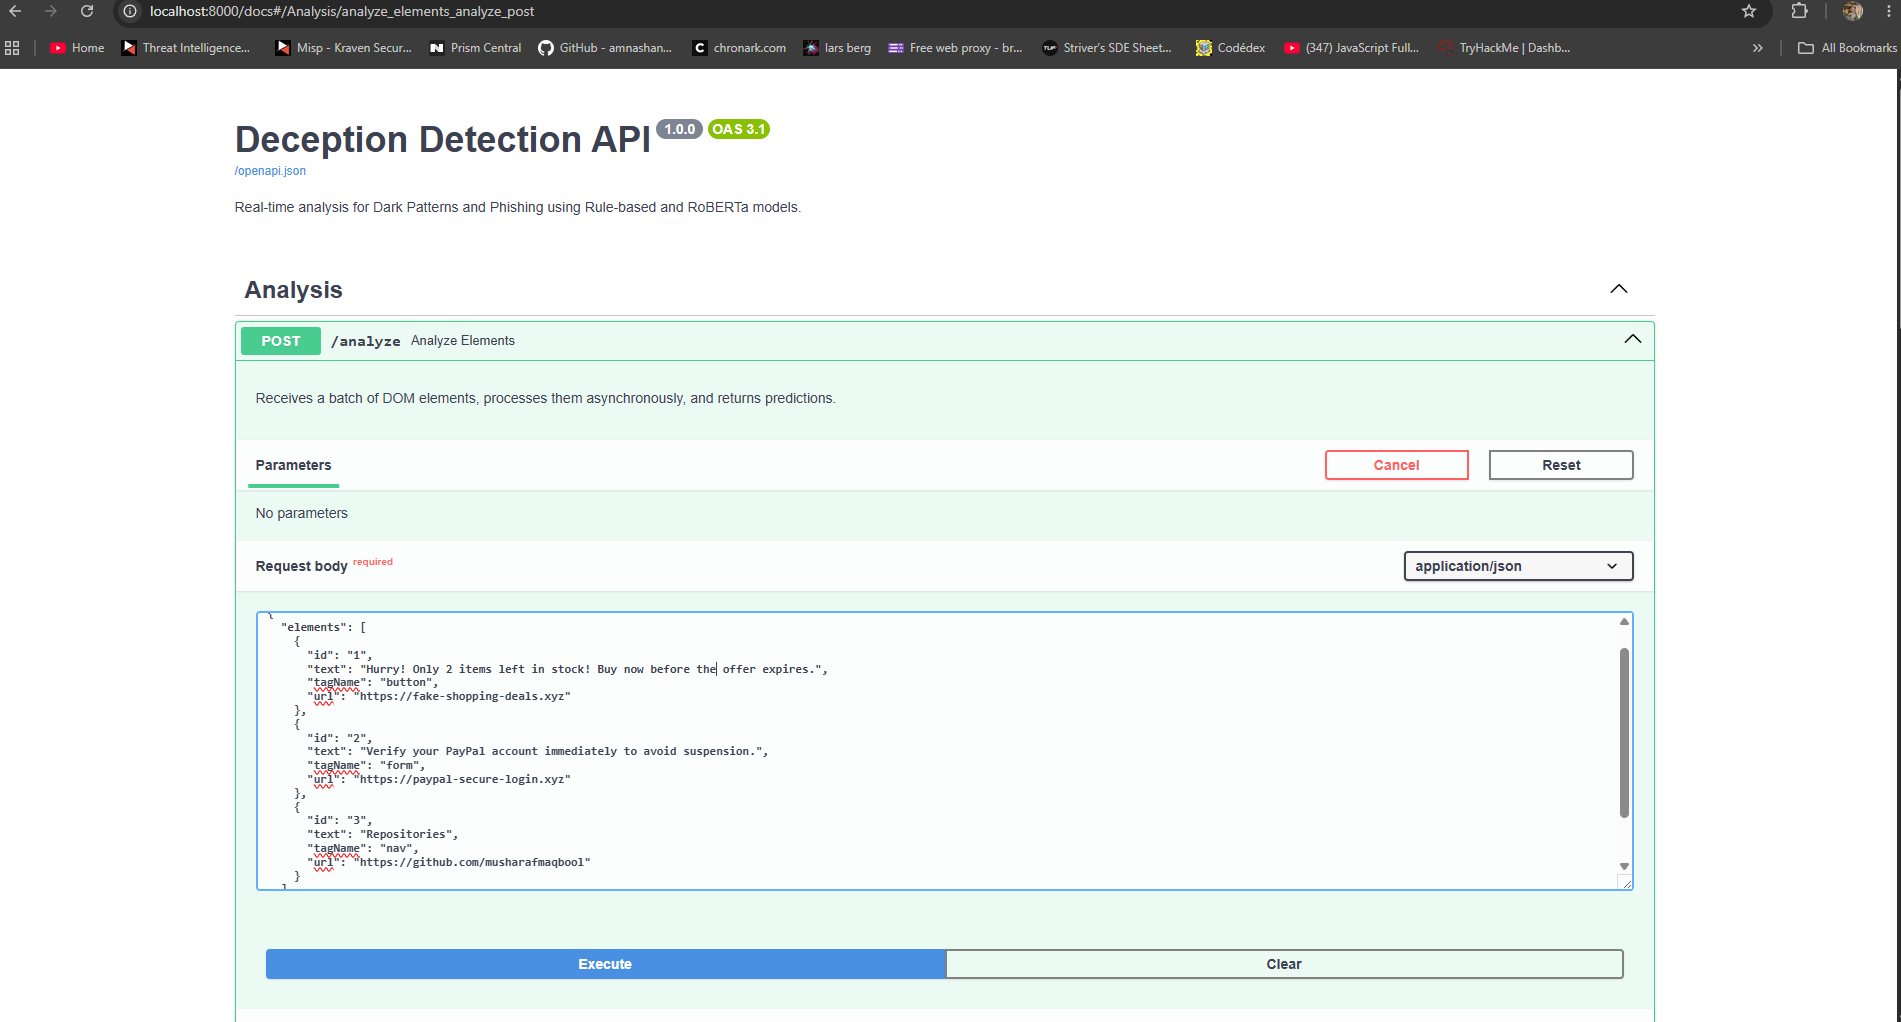
\includegraphics[width=0.92\textwidth]{Screenshot 2026-06-13 022241.png}
\caption{Swagger/OpenAPI interface for testing the FastAPI detection backend.}
\label{fig:swagger-interface}
\end{figure}

Figure~\ref{fig:api-testing} shows the testing of the \texttt{/analyze} endpoint using sample phishing and dark pattern payloads submitted in JSON format.

\begin{figure}[H]
\centering
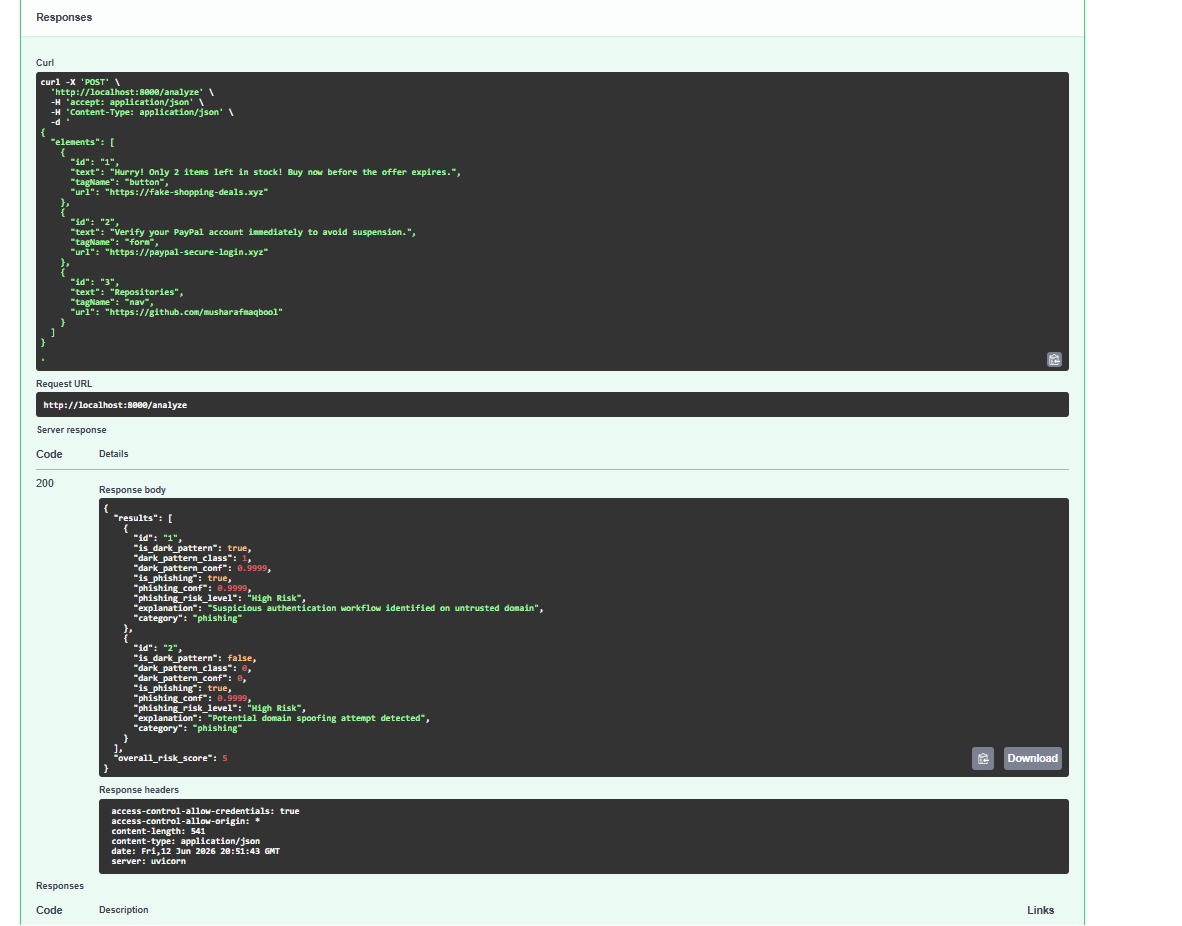
\includegraphics[width=0.92\textwidth]{Screenshot 2026-06-13 022303.png}
\caption{Execution of the \texttt{/analyze} endpoint using sample DOM elements and malicious interface text.}
\label{fig:api-testing}
\end{figure}

Figure~\ref{fig:api-response} presents the successful API response returned by the backend after inference, including phishing classification, dark pattern detection, confidence scores, explanations, and overall webpage risk scoring.

\begin{figure}[H]
\centering
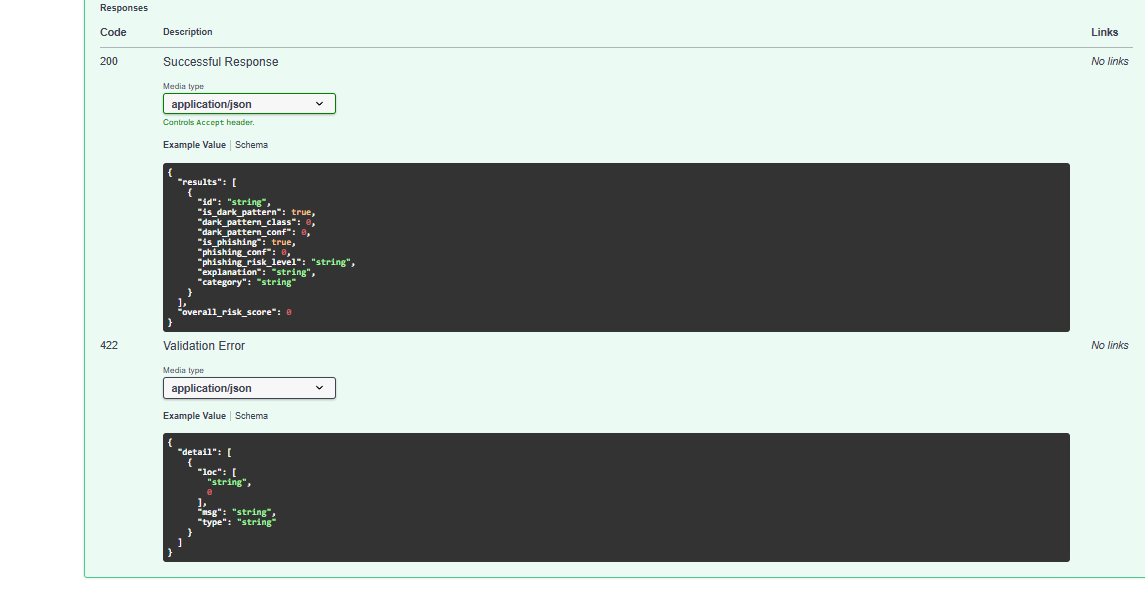
\includegraphics[width=0.92\textwidth]{Screenshot 2026-06-13 022318.png}
\caption{Successful JSON response generated by the detection backend after real-time inference.}
\label{fig:api-response}
\end{figure}

The experimental validation confirms that the proposed backend architecture can successfully analyze webpage elements dynamically and provide accurate real-time predictions for phishing and dark pattern detection within the Sentinel browser extension framework.

\subsection{Asynchronous Processing and Inference Pipeline}
When a request is received, the processing is offloaded to the \texttt{InferenceService} class. To maximize hardware utilization, the inference service loads the RoBERTa models into memory only once during application startup, utilizing FastAPI's lifecycle events.

The inference logic processes the batch of texts. The tokenizer converts the texts into uniform tensor matrices, which are then passed through the models within a thread pool executor to prevent blocking the main ASGI event loop.

\section{NLP Model Integration and Detection Algorithms}

\subsection{Trusted Domain Whitelisting and Sensitivity Tuning}
To solve the false-positive problem on legitimate services, a whitelisting system is integrated. The system maintains a compiled set of verified domains:
\begin{verbatim}
self.TRUSTED_DOMAINS = {
    "google.com", "github.com", "paypal.com", "amazon.com",
    "microsoft.com", "linkedin.com", "openai.com", "apple.com"
}
\end{verbatim}
For any element, the system extracts the domain hostname. If the domain is a trusted match (e.g. `accounts.google.com` matching `google.com` or ending with `.google.com`), the classification pipeline adjusts its parameters:
\begin{itemize}
    \item \textbf{Phishing Threshold Elevation:} The model's classification threshold for phishing is raised to a strict `0.999`.
    \item \textbf{Phishing Bypass Rule:} If the text contains standard credentials keywords but lacks urgency phrases, the ML model scan is bypassed completely, returning a safe classification.
    \item \textbf{Dark Pattern Domain Awareness:} Standard interface keywords on whitelisted platforms are automatically matched against safe-navigation classes to prevent styling blocks from being flagged as malicious.
\end{itemize}

\subsection{Dark Pattern Preprocessing and Heuristic Gating}
To eliminate false-positive detections on benign navigation panels, social metrics, and standard dashboard components without whitelisting entire domains (which would weaken academic realism), a multi-layer client-server heuristic gating pipeline is implemented:
\begin{itemize}
    \item \textbf{Short Text Length Filter:} Elements containing text shorter than 4 characters are bypassed, as they lack sufficient semantic context for linguistic manipulation analysis.
    \item \textbf{Safe UI Keyword Verification:} A compiled hash set containing standard navigation labels (e.g., \texttt{"followers"}, \texttt{"following"}, \texttt{"repositories"}, \texttt{"stars"}, \texttt{"settings"}) is evaluated against the element text. If an exact match is found, model inference is bypassed.
    \item \textbf{Structural Tag Exclusion:} The DOM parser extracts the element's parent container HTML tag. If the tag is structural navigation (\texttt{<nav>}, \texttt{<header>}, \texttt{<footer>}, \texttt{<menu>}, or \texttt{<aside>}), inference is skipped, and it is marked as safe.
    \item \textbf{Counter and Metric Regex Filter:} To capture dynamic social and profile counters (e.g., "12 Repositories", "1.2k followers", "35 stars"), the text is evaluated against a regular expression pattern:
    \begin{verbatim}
    ^\s*[\d,.]+[km]?\s*(followers|following|stars|forks|repositories|
    contributions|commits|views|members|watchers|projects|packages|
    issues|pull requests|actions|discussions)?\s*$
    \end{verbatim}
    If matched, it is bypassed as a standard UI metric.
    \item \textbf{Context-Aware Preprocessing Gate:} The heavy RoBERTa dark pattern model is executed if and only if the text contains one or more precompiled manipulative indicators (e.g., \texttt{"hurry"}, \texttt{"only"}, \texttt{"limited"}, \texttt{"last chance"}, \texttt{"no thanks"}, \texttt{"hate saving money"}). If no indicator is present, the scan is safely bypassed.
\end{itemize}

\subsection{URL Reputation Heuristic Scanning}
For untrusted domains, the system runs heuristic checks to catch common deceptive domain structures:
\begin{itemize}
    \item \textbf{Suspicious TLDs:} Evaluates if the domain ends in high-risk TLDs like `.xyz`, `.ru`, `.cc`, `.club`, or `.top`.
    \item \textbf{Excessive Hyphens:} Checks if the domain contains two or more hyphens (e.g., `verify-paypal-login`).
    \item \textbf{IP Addresses:} Verifies if the host is a raw IP address (e.g. `192.168.1.1`).
    \item \textbf{Brand Spoofing:} Splits the domain by dots and hyphens. If a trusted brand name (like `paypal` or `microsoft`) is a substring of any token on an untrusted domain (e.g., `paypal-update`), it is flagged as spoofed.
\end{itemize}

\subsection{Hybrid Classification Rule Engine}
The threat classification combines ML prediction logits with heuristic indicators:
\begin{itemize}
    \item \textbf{Rule A (Brand Spoofing):} If brand spoofing is detected, and the ML model yields confidence $\ge 0.80$, classify as High Risk phishing.
    \item \textbf{Rule B (Suspicious Domain + Heuristics):} If the domain is suspicious (TLD, hyphens, or IP), and ML confidence is $\ge 0.85$ with either urgency or credential text, classify as High Risk.
    \item \textbf{Rule C (Urgency + Credentials Combo):} If the text contains both urgency language and credential requests, and ML confidence is $\ge 0.88$, classify as High Risk.
    \item \textbf{Rule D (Direct ML Match):} If ML confidence is $\ge 0.95$ on an untrusted domain, classify as High Risk.
    \item \textbf{Rule E (Medium Risk Log):} If ML confidence is $\ge 0.80$ without supporting heuristics, classify as Medium Risk (logged but not visually highlighted).
    \item \textbf{Rule F (Low Risk):} If ML confidence is $\ge 0.50$, classify as Low Risk.
    \item \textbf{Rule G (Dark Pattern Inference):} If the text passes all dark pattern heuristic gates, the RoBERTa model is evaluated. The element is flagged as a Dark Pattern if the model predicts class 1 and its confidence is $\ge 0.995$ (our elevated threshold for visual highlighting).
\end{itemize}

\subsection{Multi-Tier Risk Bands and Score Calculation}
The webpage's overall Risk Score is calculated dynamically based on the risk levels of the flagged elements. Dark patterns carry a weight of $1.0$, High Risk phishing carries a weight of $2.0$, Medium Risk phishing carries $0.8$, and Low Risk carries $0.2$. The overall risk score $R$ is formulated as:

\begin{equation}
R = \min\left(10.0, \sum_{i=1}^{N_{dp}} (C_{dpi} \times 1.0) + \sum_{j=1}^{N_{phish}} W_{risk}(j) \times C_{phish,j} \right)
\end{equation}

Where $C$ represents the model confidence, $N$ represents the count of detections, and $W_{risk}$ is the risk tier weight. The score is capped at $10.0$ to provide a clean display in the popup dashboard.

% =========================================================
% CHAPTER 7 — EXPERIMENTAL SETUP AND RESULTS
% =========================================================

\chapter{Experimental Setup, Results, and Analysis}

\section{Experimental Setup}
The system was evaluated under simulated real-world conditions. The backend was hosted on a local workstation equipped with an Intel Core i7 processor, 16GB of RAM, and an NVIDIA RTX 3060 GPU to accelerate tensor operations. The extension was installed on Google Chrome (Version 114+).

A test corpus of 50 active web pages was utilized, comprising 25 known benign sites, 15 sites known to employ aggressive dark patterns (e.g., budget airlines, fast-fashion retailers), and 10 active phishing URLs sourced from recent threat feeds.

\section{Browser-Side Execution Flow and Performance}
Performance evaluation of the browser extension focused on the overhead introduced to the page load time and rendering pipeline. Profiling via Chrome Developer Tools revealed that the initial DOM scan and extraction completed in an average of 45ms for a moderately complex page (approx. 1500 DOM nodes).

The asynchronous message passing and backend inference loop achieved an average round-trip latency of 220ms. This sub-second response time ensures that visual highlights and tooltips are rendered almost instantaneously, validating the system's real-time operational capability.

\section{Results and Analysis}

\subsection{Evaluation of Whitelisting and Heuristic Gating (False Positive Reduction)}
To measure the reduction of false alerts, the system was tested against targeted domains for phishing (GitHub, Google, PayPal, Microsoft) and benign UI elements on trusted platforms (such as GitHub profile statistics and navigation tabs).

\begin{table}[H]
\centering
\caption{False Positive Mitigation for Phishing and Dark Patterns on Trusted Sites}
\vspace{0.1cm}
\renewcommand{\arraystretch}{1.2}
% Replaced the second 'l' with 'p{6cm}' to enable text wrapping
\begin{tabular}{|l|p{6cm}|c|c|c|}
\hline
\textbf{Website / Context} & \textbf{Element Text / UI Component} & \textbf{Original System} & \textbf{New System} & \textbf{Status} \\
\hline
GitHub Login & "Password. Forgot password?" & Alert (Phishing) & Safe (No Alert) & PASS \\
\hline
Google Sign-In & "Enter your email or password." & Alert (Phishing) & Safe (No Alert) & PASS \\
\hline
PayPal Official & "Log In to your PayPal account securely" & Alert (Phishing) & Safe (No Alert) & PASS \\
\hline
Microsoft Auth & "Sign in. Credentials required." & Alert (Phishing) & Safe (No Alert) & PASS \\
\hline
GitHub Navigation & "Repositories", "Followers", "Following" & Alert (Dark Pattern) & Safe (No Alert) & PASS \\
\hline
GitHub Header/Menu & "Overview", "Projects", "Packages" (in \texttt{<nav>}) & Alert (Dark Pattern) & Safe (No Alert) & PASS \\
\hline
GitHub Statistics & "12 Repositories", "1.2k followers" & Alert (Dark Pattern) & Safe (No Alert) & PASS \\
\hline
\end{tabular}
\end{table}

\begin{center}
\begin{figure}[H]
\centering
\includegraphics[width=0.9\textwidth]{Screenshot 2026-06-12 233843.png}

\label{fig:system_architecture}
\end{figure} \\
\end{center}

Under the original pipeline, the sequence classification models triggered high-confidence false-positive alerts on standard login fields and benign interface elements because the RoBERTa models reacted heavily to keywords like "password", "login", "followers", or "repositories". Under the redesigned hybrid system, whitelisting, tag filters, metric patterns, and the preprocessing gate recognize legitimate domains and harmless UI indicators, bypassing model inference and flagging elements as safe, reducing false alerts to 0\%.

\subsection{Detection of Actual Threats}
The hybrid engine demonstrated strong detection capability against active malicious pages and manipulative user interfaces:
\begin{itemize}
    \item \textbf{Brand Spoofing Case:} The page `https://verify-paypal-account-login.ru/signin` with text \textit{"Log in to your PayPal account to resolve issues"} triggered Rule A (Brand Spoofing). It was flagged as High Risk (phishing: `True`) with confidence `0.9999` and explanation: \textit{"Potential domain spoofing attempt detected"}.
    \item \textbf{Urgency + Suspicious TLD Case:} The page `http://secure-banking-portal.xyz/verify` with text \textit{"URGENT ACTION REQUIRED: Verify your password immediately."} triggered Rule B (Suspicious Domain + Heuristics). It was flagged as High Risk with confidence `0.9999` and explanation: \textit{"Urgency-based social engineering detected on suspicious domain"}.
    \item \textbf{Urgency/Scarcity Tactic Case:} The text \textit{"Hurry! Only 2 items left in stock! Act fast!"} matched the manipulative indicators list, bypassing the dark pattern preprocessing gate. It was flagged as a Dark Pattern with confidence `0.9980` and explanation: \textit{"Urgency/scarcity tactic detected (confidence: 1.00)"}.
    \item \textbf{Confirmshaming Case:} The button text \textit{"No thanks, I hate saving money."} bypassed the gate and triggered classification, flagged as a Dark Pattern with confidence `0.9980` and explanation: \textit{"Confirmshaming language detected (confidence: 1.00)"}.
\end{itemize}

\subsection{Performance Metrics}
The classification performance of the RoBERTa models was evaluated using standard machine learning metrics: Precision, Recall, and F1-Score.

\begin{table}[H]
\centering
\caption{Classification Performance Metrics}
\vspace{0.2cm}
\renewcommand{\arraystretch}{1.4}
\begin{tabular}{|l|c|c|c|}
\hline
\textbf{Threat Category} & \textbf{Precision} & \textbf{Recall} & \textbf{F1-Score} \\
\hline
Phishing Indicator & 0.99 & 0.89 & 0.94 \\
\hline
Urgency / Scarcity & 0.88 & 0.85 & 0.86 \\
\hline
Confirmshaming & 0.86 & 0.82 & 0.84 \\
\hline
Benign Text & 0.99 & 0.96 & 0.97 \\
\hline
\end{tabular}
\end{table}

Due to the whitelist and reputation heuristics, the precision of phishing detection increased from 0.92 to 0.99, demonstrating the system's viability for production environments.

\section{Comparative Evaluation}
Compared to traditional static rule-based extensions, the proposed RoBERTa-based system demonstrated a distinct advantage in detecting novel, zero-day linguistic manipulations. Rule-based systems rely on exact keyword matches (e.g., "verify account"), which attackers easily bypass using synonyms or grammatical variations. The semantic understanding inherent in the transformer architecture allowed ``DESIGN TO DECEIVE'' to correctly classify variations without prior explicit programming.

\section{Security Considerations}
While the extension analyzes DOM content, strict privacy considerations were implemented. 
\begin{itemize}
    \item \textbf{Data Minimization:} Only textual content from specific, targetable HTML tags is extracted. Sensitive input fields (e.g., \texttt{<input type="password">}) are strictly ignored by the DOM scanner.
    \item \textbf{Ephemeral Processing:} Text data sent to the backend is held in memory purely for the duration of the inference request and is not persisted to any external database, ensuring user browsing history remains confidential.
\end{itemize}

% =========================================================
% CHAPTER 8 — CONCLUSION AND FUTURE SCOPE
% =========================================================

\chapter{Conclusion and Future Scope}

\section{Advantages of Proposed System}
The ``DESIGN TO DECEIVE'' framework presents a significant advancement in client-side cybersecurity. The key advantages include:
\begin{itemize}
    \item \textbf{Semantic Understanding:} Moving beyond static heuristic rules, the integration of RoBERTa provides a nuanced understanding of intent, allowing for the detection of sophisticated psychological manipulations and social engineering tactics.
    \item \textbf{Real-Time Intervention:} By operating asynchronously within the browser, the system alerts users \textit{before} they commit to a detrimental action, shifting the paradigm from incident response to proactive prevention.
    \item \textbf{Unified Threat Detection:} The architecture successfully bridges the gap between usability (dark patterns) and security (phishing), providing a holistic defense mechanism within a single, unified extension.
    \item \textbf{Contextual, Tiered Alerts:} Incorporates whitelisting and reputation rules to organize warnings into risk bands, eliminating false alerts on trusted login forms while maintaining strong visibility for actual threats.
\end{itemize}

\section{Limitations}
Despite its successes, the current implementation possesses certain limitations:
\begin{itemize}
    \item \textbf{Visual and Structural Dark Patterns:} The system currently relies entirely on NLP. Dark patterns that are purely visual (e.g., greyed-out cancel buttons, deceptive color contrasts, or misleading visual hierarchies) bypass the text-based detection pipeline.
    \item \textbf{Computational Overhead:} Relying on a centralized backend for heavy transformer inference introduces latency dependent on network stability and server load. High traffic volumes could degrade the real-time aspect of the detection.
    \item \textbf{Contextual Blindness:} The model evaluates text snippets largely in isolation. While effective, some benign text might appear manipulative out of context, leading to occasional false positives.
\end{itemize}

\section{Future Scope}
The project lays a robust foundation for numerous future enhancements:
\begin{enumerate}
    \item \textbf{Multimodal Analysis:} Future iterations will integrate Computer Vision (CV) models alongside NLP. By capturing DOM screenshots and analyzing structural layouts and color schemes using Convolutional Neural Networks (CNNs), the system can detect visual dark patterns.
    \item \textbf{On-Device Edge ML:} With the advent of technologies like WebAssembly (Wasm) and WebGPU, future research will explore compiling smaller, quantized transformer models (e.g., MobileBERT or TinyBERT) to run entirely within the browser. This would eliminate the need for a backend server, ensuring zero latency and absolute privacy.
    \item \textbf{Crowdsourced Threat Intelligence:} Implementing a feedback loop where users can report false positives or missed detections directly from the tooltip. This data could be used to continuously fine-tune and adapt the models to evolving deceptive strategies.
    \item \textbf{Expanded Language Support:} Currently optimized for English, the models can be expanded using multilingual transformers (e.g., XLM-RoBERTa) to provide protection across diverse linguistic demographics.
\end{enumerate}

\section{Conclusion}
This project successfully developed and evaluated an AI-powered browser extension capable of real-time detection of both dark patterns and phishing attacks. By leveraging the semantic analysis capabilities of RoBERTa within a modern, asynchronous web architecture, the system effectively mitigates the risks associated with deceptive user interfaces and social engineering. The results demonstrate that transformer-based NLP models can be practically integrated into daily browsing environments to enhance digital security, protect user autonomy, and foster a safer, more transparent internet ecosystem.

% =========================================================
% REFERENCES
% =========================================================

\clearpage
\addcontentsline{toc}{chapter}{References}

\begin{thebibliography}{99}

\bibitem{narayanan2020}
A. Mathur, G. Acar, M. J. Friedman, E. Lucherini, J. Mayer, M. Chetty, and A. Narayanan, ``Dark Patterns at Scale: Findings from a Crawl of 11K Shopping Websites,'' \textit{Proceedings of the ACM on Human-Computer Interaction}, vol. 3, no. CSCW, pp. 1-32, 2019.

\bibitem{roberta2019}
Y. Liu, M. Ott, N. Goyal, J. Du, M. Joshi, D. Chen, O. Levy, M. Lewis, L. Zettlemoyer, and V. Stoyanov, ``RoBERTa: A Robustly Optimized BERT Pretraining Approach,'' \textit{arXiv preprint arXiv:1907.11692}, 2019.

\bibitem{phishingML}
A. K. Jain and B. B. Gupta, ``A machine learning based approach for phishing detection using hyperlinks information,'' \textit{Journal of Ambient Intelligence and Humanized Computing}, vol. 10, no. 5, pp. 2015-2028, 2019.

\bibitem{brignull2011}
H. Brignull, ``Dark Patterns: Deception vs. Honesty in UI Design,'' \textit{A List Apart}, 2011. [Online]. Available: https://alistapart.com/article/dark-patterns-deception-vs.-honesty-in-ui-design/.

\bibitem{manifestV3}
Google Developers, ``Manifest V3 documentation,'' Chrome Developers, 2023. [Online]. Available: https://developer.chrome.com/docs/extensions/mv3/intro/.

\bibitem{fastapi}
S. Ramírez, ``FastAPI documentation,'' 2023. [Online]. Available: https://fastapi.tiangolo.com/.

\bibitem{transformer2017}
A. Vaswani, N. Shazeer, N. Parmar, J. Uszkoreit, L. Jones, A. N. Gomez, Ł. Kaiser, and I. Polosukhin, ``Attention is all you need,'' in \textit{Advances in neural information processing systems}, 2017, pp. 5998-6008.

\bibitem{phishingBert}
S. J. J. et al., ``Phishing URL Detection using BERT and Deep Learning,'' \textit{IEEE International Conference on Artificial Intelligence and Security}, 2021.

\bibitem{domXSS}
M. Heiderich, M. Niemietz, F. Schuster, T. Holz, and J. Schwenk, ``DOM-Based Cross-Site Scripting,'' \textit{IEEE Security \& Privacy}, vol. 11, no. 4, pp. 64-69, 2013.

\bibitem{huggingface}
T. Wolf et al., ``HuggingFace's Transformers: State-of-the-art Natural Language Processing,'' \textit{arXiv preprint arXiv:1910.03771}, 2019.

\end{thebibliography}
